% !TeX program = pdflatex
%=======================================================================
% RG-SCSO, Springer Nature (sn-jnl) format, target: Iranian Journal of
% Computer Science (IJCS). Forked from the Elsevier/elsarticle (ASOC)
% version; same body content throughout, only the class/frontmatter/
% back-matter differ per IJCS's own submission-guidelines page
% (link.springer.com/journal/42044/submission-guidelines): documentclass
% option [iicol,sn-basic,pdflatex], bibliography style sn-basic.bst.
% Font: newtxtext/newtxmath (Times-like, pdflatex-compatible) -- NOT
% fontspec/unicode-math (those need XeLaTeX/LuaLaTeX; IJCS's own
% guidelines specify the [pdflatex] class option, i.e. the standard pdfTeX
% engine).
%=======================================================================
\documentclass[iicol,sn-basic,pdflatex]{sn-jnl}
\usepackage{newtxtext,newtxmath}
\usepackage{amsmath}
\usepackage{amsthm}
\usepackage{algorithm}
\usepackage{algorithmic}
\usepackage{graphicx}
\graphicspath{{figures/}{./}}
\usepackage{booktabs}
\usepackage{multirow}
\usepackage{rotating}
\usepackage{url}
\usepackage{placeins}
\raggedbottom
\makeatletter
\setlength{\@fptop}{0pt}
\setlength{\@fpsep}{12pt}
\setlength{\@fpbot}{0pt plus 1fil}
\makeatother
\renewcommand{\topfraction}{0.95}
\renewcommand{\floatpagefraction}{0.85}
\renewcommand{\bottomfraction}{0.9}
\renewcommand{\textfraction}{0.05}
\setcounter{topnumber}{4}
\setcounter{bottomnumber}{4}
\setcounter{totalnumber}{8}

\newtheorem{lemma}{Lemma}
\newtheorem{proposition}[lemma]{Proposition}

\begin{document}

\title[RG-SCSO for Parsimonious Feature Selection]{Relevance-Guided
Binarization for Parsimonious Feature Selection with Sand Cat Swarm
Optimization}

\author*[1]{\fnm{Bui Quang} \sur{Huy}}\email{huybq@donga.edu.vn}
\author[1]{\fnm{Duong Minh} \sur{Son}}\email{sondm@donga.edu.vn}
\affil[1]{\orgname{Dong A University}, \city{Da Nang}, \country{Vietnam}}

\abstract{Wrapper feature selection with swarm intelligence typically searches in continuous space and crosses into the binary domain through a fixed transfer function, a feature-agnostic quantization that discards the continuous operators' fine adjustments, an effect we term washout. RG-SCSO replaces this transfer with a per-feature, relevance-modulated binarization: a mutual-information field biases each feature's bit-flip probability so informative features resist removal and noise resists inclusion, leaving SCSO's continuous search otherwise unchanged. Evaluated on 18 datasets, including two gene-expression sets, under a budget-matched, leak-free protocol that computes the relevance prior, the search, and the cross-validated fitness only on the training partition, RG-SCSO attains the best mean held-out accuracy of the seven metaheuristics compared while selecting the second-smallest feature subsets of any method tested, trailing only COA, which is several points less accurate. The advantage is parsimony rather than raw accuracy: it persists against optimizers carrying published adaptive transfers, against which RG-SCSO still selects 26--43\% fewer features, and against same-family binary SCSO selectors; ablation and cross-prior tests show it depends on where the relevance signal is injected and on the prior used. On the two gene-expression sets a classical LASSO baseline is sparser at no loss of accuracy, so the transferable gain is parsimony on data without that extreme structure.}

\keywords{Feature selection, Sand Cat Swarm Optimization, binary
optimization, relevance-guided binarization, parsimony}

\maketitle

\FloatBarrier
\section{Introduction}
Feature selection removes irrelevant and redundant features to improve
classifier accuracy, reduce overfitting, and lower computational cost, a
payoff that is greatest for high-dimensional, small-sample problems such as
gene-expression classification, where the number of features exceeds the
number of samples by orders of magnitude~\cite{guyon,mrmr}. Wrapper
selection, which scores a subset by the performance of a downstream
classifier, is frequently cast as a combinatorial problem solved by
swarm-intelligence metaheuristics, including grey wolf~\cite{bgwo}, particle
swarm~\cite{pso}, whale~\cite{mafarja}, and several recent
optimizers~\cite{aoa,coa,rime}. Most such methods were conceived for
continuous optimization and are adapted to the binary space through a
transfer function, most commonly an S-shaped or V-shaped map, that converts a
real-valued position into a selection probability~\cite{tf}. We argue that
this retrofit contains a structural weakness: the transfer function is fixed
and feature-agnostic, applied identically to every dimension, so the
incremental adjustments a continuous-space operator makes are collapsed by
the squash-and-threshold step before they can influence the retained subset.
We refer to this loss as washout, and show in Methods below that it is not a
thought experiment: four well-motivated continuous-space enhancements of
SCSO~\cite{scso} failed to beat the base algorithm under an identical
feature-selection protocol (0 wins, 1 loss, 17 ties by Wilcoxon signed-rank;
Supplementary Table~S5, preliminary washout study).

Existing studies have explored relevance-guided initialization, objective
weighting, and adaptive binary transfer mechanisms; however, the explicit
injection of a per-feature relevance prior into the binarization operator of
SCSO-based feature selection remains insufficiently investigated
(Section~\ref{sec:relwork} positions this gap against each cited
SCSO-family work in detail).

We close this gap with RG-SCSO: a per-feature, relevance-modulated
binarization in which a mutual-information relevance field biases each
feature's bit-flip probability, turning a knowledge-agnostic quantization
step into a knowledge-carrying operator. SCSO's continuous search, including
its sensitivity range, is retained unchanged; the novelty resides entirely in
the binarization (Fig.~\ref{fig:concept}). This paper makes four
contributions. First, we identify washout as a mechanistic failure mode and
derive a diagnostic bound, together with a cumulative extension linking it to
discrete transition dynamics. Second, we propose RG-SCSO, whose
ablation-confirmed centerpiece is relevance-modulated sensitivity (RMS),
supplemented by a smaller, budget-neutral memetic refinement step (UMR) that a
sensitivity sweep shows contributes far less than RMS; an online-learning
variant of the relevance field is examined and pruned entirely by ablation.
Third, we evaluate under a preregistered, budget-matched, leak-free protocol
that denies the relevance prior any access to test labels. Fourth, we report a
full statistical treatment, a component ablation, and a size-fair enrichment
analysis correlating the observed parsimony with relevance guidance.

\subsection{Research questions}
This study is organized around four research questions, each answered
directly by a specific part of Results or Discussion below.
\begin{itemize}
\item \textbf{RQ1.} Does relevance-modulated binarization improve held-out
  feature-selection performance under a fixed computational budget?
  \emph{Addressed in Section~\ref{sec:heldout} (Table~\ref{tab:heldout},
  Fig.~\ref{fig:cd}).}
\item \textbf{RQ2.} Can RG-SCSO reduce the number of selected features while
  preserving competitive generalization accuracy?
  \emph{Addressed in Section~\ref{sec:parsimony}.}
\item \textbf{RQ3.} Is direct relevance injection at the binarization
  interface more effective than relevance-guided initialization or
  objective weighting?
  \emph{Addressed in Section~\ref{sec:ablation} (Table~\ref{tab:ablation}).}
\item \textbf{RQ4.} How robust is the proposed mechanism across
  classifiers, relevance priors, and dataset dimensionalities?
  \emph{Addressed in Section~\ref{sec:classical}
  (Table~\ref{tab:classifierrobust}) and Discussion.}
\end{itemize}

The remainder of the paper reviews existing approaches along three axes: (i)
binary transfer functions in swarm-based feature selection, (ii)
relevance-guided search mechanisms, and (iii) SCSO variants
(Section~\ref{sec:relwork}).

\begin{figure}[htbp]
\centering
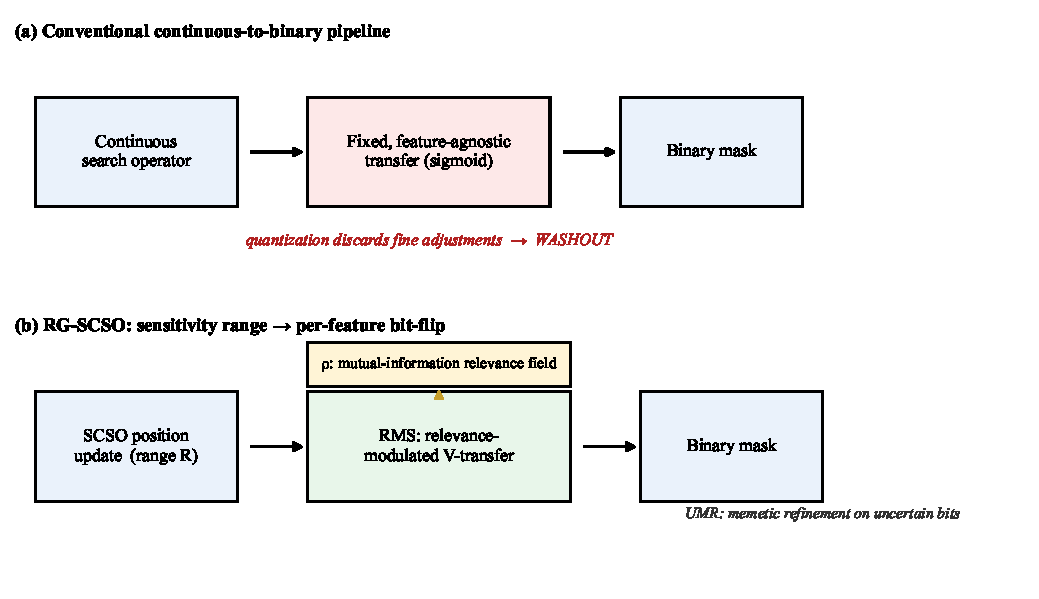
\includegraphics[width=0.92\textwidth]{concept.pdf}
\caption{Conceptual overview. (a) The conventional pipeline, where
continuous-operator adjustments are collapsed by a fixed, feature-agnostic
transfer (washout). (b) RG-SCSO, where a per-feature, relevance-modulated
binarization replaces the feature-agnostic transfer, biasing each feature's
bit-flip probability by a mutual-information relevance field, followed by
memetic refinement on uncertain bits.}
\label{fig:concept}
\end{figure}

\FloatBarrier
\section{Related work}
\label{sec:relwork}
\subsection{Binary transfer functions in swarm-based feature selection}
Swarm-intelligence wrapper selectors, including grey wolf~\cite{bgwo},
particle swarm~\cite{pso}, whale~\cite{mafarja}, and several recent
optimizers~\cite{aoa,coa,rime}, are conceived for continuous optimization
and cross into the binary search space through a transfer function, most
commonly an S-shaped or V-shaped map~\cite{tf}. A substantial recent line of
work makes this interface \emph{adaptive} rather than static: time-varying
transfer functions that reshape the squashing curve as the search
progresses~\cite{islam2017tvtf,bgoatvg2024}, and fitness- or history-driven
schemes that tune it from the swarm's own progress~\cite{teng2017avbpso,fhsbpso2024}.
Crucially, all of these remain \emph{feature-agnostic}: the same (possibly
time-varying) transfer is applied identically to every dimension regardless
of that feature's relevance, the structural weakness this paper terms washout
(Introduction, Methods). RG-SCSO is orthogonal to this line -- it modulates
the binarization per feature by a relevance prior, and could in principle be
combined with an adaptive transfer rather than replacing one.

\subsection{Relevance-guided mechanisms in feature selection}
Filter criteria such as mutual information and mRMR~\cite{guyon,mrmr} encode
problem knowledge cheaply but are decoupled from the wrapper search; memetic
hybridization~\cite{neri} adds local refinement without addressing the
binarization interface. A large family of knowledge-guided metaheuristics
injects filter information \emph{upstream} of the binary decision, into
initialization or the objective. In other swarm families this takes the form
of correlation- or mutual-information-guided population
initialization~\cite{mobgwogms2023,hhoelm2023}, filter-guided PSO for
cancer-genome selection~\cite{ludwig2025guided}, and memetic hybridization
of binary Harris-hawks and whale operators~\cite{whalehho2022}; a parallel,
deep-learning-oriented direction drives selection from post-hoc attribution
or attention, for example SHAP-guided deep feature
selection~\cite{xaifs2024}. All of these bias \emph{where} the search
starts, \emph{what} it optimizes, or which features a separately trained
model highlights, yet leave the binarization operator itself
knowledge-agnostic. RG-SCSO differs by injecting the relevance signal at the
binarization interface itself rather than upstream of it; the signal-position
experiment in Results (Table~\ref{tab:ablation}) tests this design choice
directly against both the initialization and objective alternatives.

\paragraph{Positioning against relevance-injecting binary GWO/WOA/HHO
variants.} The closest competitors are binary grey-wolf, whale, and
Harris-hawks selectors that already carry a relevance signal: MOBGWO-GMS
initializes its population from feature correlation and guides mutation with
it~\cite{mobgwogms2023}, the enhanced Harris-hawks optimizer seeds the search
with filter-ranked features~\cite{hhoelm2023}, and hybrid binary
whale/Harris-hawks memetics combine two operators for stronger local
search~\cite{whalehho2022}. Each injects relevance at initialization,
mutation, or hybridization; none makes the \emph{per-feature binarization
operator} itself relevance-aware, which is the specific interface RG-SCSO
modifies and the reason its parsimony gain (Results) is not reproduced by
these variants' upstream injections.

\subsection{Sand Cat Swarm Optimization and its variants}
SCSO~\cite{scso} is a comparatively recent continuous metaheuristic. The
existing binary SCSO feature selectors~\cite{bscso,scsofs2,scsofs3} apply
standard transfer functions without a relevance-aware binarization step, and
the broader recent SCSO literature that adds chaotic initialization,
differential mutation, or hybridized search
strategies~\cite{imscso2024,mescso2025,scsolensobl2024,improvedscso2024}
improves continuous-space search dynamics while leaving the binarization
interface itself untouched -- none of these works, to our knowledge, makes
the binarization operator itself per-feature and relevance-aware.
Table~\ref{tab:litpos} below positions each of these works against this
claim directly.

\subsection{Literature-positioning summary}
Table~\ref{tab:litpos} makes this gap concrete across every SCSO-family
work cited above: the three directly comparable binary feature selectors
apply a standard, feature-agnostic transfer with no relevance-aware step,
and the four continuous-search variants improve exploration/exploitation
dynamics without touching the binarization interface at all. None of the
eight prior works positioned here makes the binarization operator itself
per-feature and relevance-aware -- the interface RG-SCSO modifies.

\begin{table}[t]
\centering
\caption{Positioning of RG-SCSO against recent SCSO-family literature cited in this paper. The four 2024--2025 continuous-search variants (IMSCSO, SCSO+Lens-OBL+SSA, Improved SCSO, MESCSO) improve exploration/exploitation dynamics in continuous space but are global optimization studies, not feature selectors, so they are not directly comparable under this paper's binary FS protocol; they are cited to establish that none of them touches the binarization interface itself. The three binary SCSO feature selectors (bSCSO and two further variants) are directly comparable and are included as same-family baselines (Discussion; Supplementary Information).}
\label{tab:litpos}
\footnotesize
\begin{tabular}{p{4.2cm}cp{3.6cm}p{3.6cm}}
\toprule
Method & Year & What it modifies & Comparable to this protocol? \\
\midrule
Seyyedabbasi \& Kiani~\cite{scso} & 2022 & Base continuous SCSO (no FS) & Baseline (Table~1) \\
bSCSO~\cite{bscso} & 2023 & Binary wrapper FS, standard transfer & Same-family baseline (Discussion) \\
Binary SCSO (biomedical)~\cite{scsofs2} & 2023 & Binary wrapper FS, standard transfer & Same-family baseline (Discussion) \\
Adaptive SCSO~\cite{scsofs3} & 2024 & Binary wrapper FS, standard transfer & Same-family baseline (Discussion) \\
IMSCSO~\cite{imscso2024} & 2024 & Continuous search (multi-strategy) & No -- global optimization only, no FS \\
SCSO+Lens-OBL+SSA~\cite{scsolensobl2024} & 2024 & Continuous search (lens-OBL init) & No -- global optimization only, no FS \\
Improved SCSO~\cite{improvedscso2024} & 2024 & Continuous search dynamics & No -- global optimization only, no FS \\
MESCSO~\cite{mescso2025} & 2025 & Continuous search (multi-strategy) & No -- global optimization only, no FS \\
\bottomrule
\end{tabular}
\end{table}


\FloatBarrier
\section{Results}
\subsection{Held-out generalization}
\label{sec:heldout}
RQ1 asks whether relevance-modulated binarization improves held-out
performance under a fixed computational budget; this subsection answers it
directly. For each dataset, algorithm, and independent run we draw an outer
stratified 80/20 split. The relevance prior, the search, and the
cross-validated fitness are computed exclusively on the 80\% training
partition; the selected subset is evaluated once on the untouched 20\%
hold-out, on which a fresh $k$-NN classifier (standardized on the training
partition) reports accuracy, so the relevance prior never has transductive
access to the test labels. Table~\ref{tab:heldout} reports held-out
accuracy over all seven algorithms and 18 datasets, at a fixed
evaluation budget of $\mathrm{max\_nfe}=15000$ for every algorithm compared.
RG-SCSO attains the best average Friedman rank (1.33, ahead of
the second-placed AOA at 2.03; $\chi^2$=66.16,
$p<10^{-3}$). A
Holm-corrected Wilcoxon signed-rank test across all pairwise comparisons gives
RG-SCSO 64 significant wins, 1 loss, and 43 ties; the only close
competitor is AOA, against which the advantage is genuine but moderate
(median $|d|=0.30$), RG-SCSO still leading on mean accuracy.
Fig.~\ref{fig:cd} visualizes this held-out ranking as a critical-difference
diagram: the Nemenyi test, a more conservative simultaneous comparison than
the pairwise Wilcoxon test above, does not separate RG-SCSO from AOA, but
places both above a single indistinguishable cluster comprising the
remaining five algorithms.

\begin{table}[t]
\centering
\caption{Held-out generalization: mean accuracy, with mean number of selected features in parentheses, on the outer 20\% hold-out over 30 runs (relevance prior, search, and CV fitness fit on the 80\% training split only; dataset feature counts are given in Supplementary Table~S1). Standard deviations are omitted here for compactness; per-run raw results, from which they can be recomputed exactly, are in the public repository (Data availability). \textbf{Bold} = best accuracy per dataset.}
\label{tab:heldout}
\tiny
\setlength{\tabcolsep}{1.0pt}
\begin{tabular}{lccccccc}
\toprule
Dataset & RG-SCSO & AOA & COA & SCSO & RIME & PSO & GWO \\
\midrule
BreastEW & 0.9630 (5.2) & \textbf{0.9679 (8.7)} & 0.9487 (4.7) & 0.9509 (4.4) & 0.9521 (3.9) & 0.9428 (4.8) & 0.9511 (4.1) \\
ColonCancer & \textbf{0.7615 (555.1)} & 0.7410 (1958.2) & 0.7205 (484.3) & 0.7410 (1002.3) & 0.7308 (999.3) & 0.7333 (1006.6) & 0.7513 (1007.0) \\
Diabetes & 0.7229 (4.6) & \textbf{0.7279 (7.4)} & 0.7000 (4.7) & 0.7030 (4.1) & 0.6883 (3.4) & 0.6695 (3.9) & 0.6708 (3.9) \\
GermanCredit & 0.7260 (8.4) & \textbf{0.7353 (19.9)} & 0.6832 (10.8) & 0.7038 (10.0) & 0.7048 (9.8) & 0.6980 (10.5) & 0.6948 (9.7) \\
HeartDisease & 0.8089 (5.9) & \textbf{0.8261 (12.8)} & 0.7833 (6.8) & 0.7661 (6.6) & 0.7633 (6.3) & 0.7367 (6.6) & 0.7567 (6.3) \\
IonosphereEW & \textbf{0.8864 (8.0)} & 0.8418 (33.9) & 0.8507 (11.0) & 0.8549 (16.5) & 0.8531 (15.8) & 0.8418 (16.6) & 0.8385 (16.5) \\
KrVsKpEW & \textbf{0.9518 (12.2)} & 0.9289 (35.0) & 0.8354 (17.3) & 0.8351 (17.5) & 0.7808 (16.4) & 0.7908 (17.1) & 0.7120 (17.2) \\
Leukemia & \textbf{0.9733 (957.4)} & 0.9622 (3549.2) & 0.9467 (623.0) & 0.9533 (1770.7) & 0.9644 (1778.9) & 0.9600 (1780.8) & 0.9578 (1788.6) \\
Lymphography & 0.7978 (7.0) & \textbf{0.8167 (17.9)} & 0.7722 (9.8) & 0.7711 (9.1) & 0.7556 (8.7) & 0.7611 (8.6) & 0.7356 (8.0) \\
M-of-n & \textbf{0.9960 (6.3)} & 0.8712 (12.8) & 0.7892 (7.1) & 0.7733 (7.2) & 0.7480 (6.6) & 0.7263 (6.1) & 0.6985 (6.2) \\
Parkinsons & \textbf{0.9051 (6.6)} & 0.9026 (21.7) & 0.8889 (8.8) & 0.8812 (11.2) & 0.8812 (10.8) & 0.8718 (11.0) & 0.8761 (10.8) \\
Sonar & \textbf{0.8079 (16.7)} & 0.8024 (59.9) & 0.7937 (28.2) & 0.7976 (29.6) & 0.7897 (29.7) & 0.7944 (30.6) & 0.8024 (29.8) \\
SpectEW & \textbf{0.8204 (7.8)} & 0.8099 (21.4) & 0.8012 (9.4) & 0.8012 (11.0) & 0.7951 (10.0) & 0.8074 (11.0) & 0.7932 (10.8) \\
TicTacToe & \textbf{0.8212 (7.7)} & 0.7856 (8.4) & 0.6924 (5.9) & 0.6462 (4.5) & 0.6538 (4.8) & 0.6552 (4.6) & 0.6241 (4.1) \\
Vote & \textbf{0.9560 (3.0)} & 0.9220 (15.9) & 0.8965 (5.2) & 0.8837 (6.5) & 0.9028 (7.9) & 0.8915 (7.2) & 0.9021 (8.3) \\
WDBC & \textbf{0.9667 (12.5)} & 0.9649 (29.7) & 0.9582 (13.7) & 0.9561 (14.9) & 0.9558 (15.0) & 0.9532 (14.5) & 0.9544 (15.0) \\
WaveformEW & \textbf{0.8153 (15.8)} & 0.7571 (38.3) & 0.7505 (21.8) & 0.7352 (20.6) & 0.7170 (20.2) & 0.7238 (20.8) & 0.6863 (19.0) \\
Zoo & 0.9079 (7.8) & \textbf{0.9190 (15.7)} & 0.8651 (9.0) & 0.8540 (8.3) & 0.8460 (8.0) & 0.8476 (8.3) & 0.8270 (7.8) \\
\bottomrule
\end{tabular}
\end{table}


\subsection{Feature-subset parsimony}
\label{sec:parsimony}
RQ2 asks whether RG-SCSO can reduce feature count while preserving
competitive accuracy; this subsection answers it directly. Parsimony, more
than any accuracy margin, is RG-SCSO's defining property.
Table~\ref{tab:heldout} shows it attains the best mean accuracy of any
method tested (0.866) while selecting the
second-fewest features on the held-out setting, on average
91.6 against
164.2 for base SCSO and
325.9 for AOA. Only COA selects fewer
(71.2 on average), and it does so at
0.051 lower
mean accuracy, so RG-SCSO is the most compact method that does not trade
away accuracy to get there. On ColonCancer it retains
563 of 2000 features
versus 1991 for AOA, at higher accuracy.
This advantage survives every stress test we run: against optimizers
carrying published adaptive transfers RG-SCSO does not lead on accuracy yet
still selects 26--43\% fewer
features, and against same-family binary SCSO
selectors~\cite{bscso,scsofs2,scsofs3} it is
42\% smaller at comparable accuracy. The dimensionality reductions are too small relative to these datasets' modest sample counts (50--455 training instances) for a wall-clock inference saving to be resolvable above call overhead; a projected, reconstructed inference-cost analysis at a synthetic deployment-scale workload, a controlled complexity demonstration rather than a measurement on the benchmark's own test sets, is reported in Supplementary Information instead of here.

\begin{figure}[htbp]
\centering
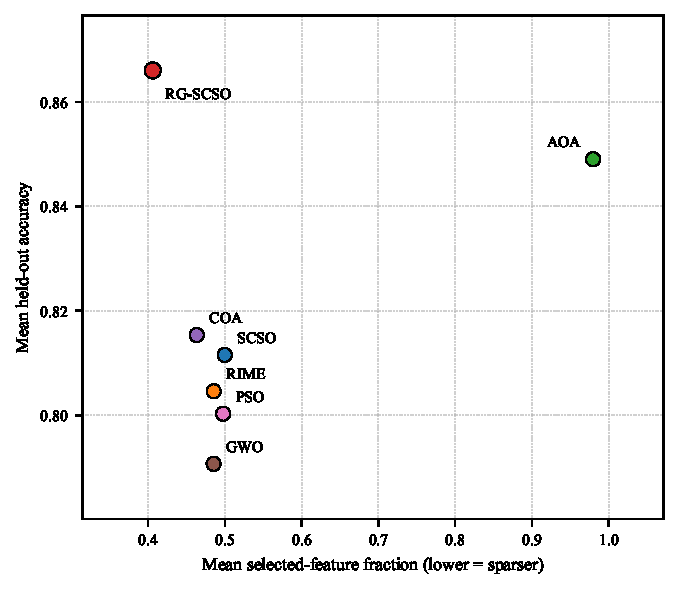
\includegraphics[width=0.7\textwidth]{accuracy_parsimony_tradeoff.pdf}
\caption{Mean held-out accuracy vs.\ mean selected-feature fraction,
averaged across all 18 datasets, one point per algorithm. RG-SCSO
occupies the top-left corner, jointly the highest accuracy and the sparsest
subsets of all seven algorithms tested -- it is not merely competitive on
one axis at the cost of the other. AOA attains the second-highest accuracy
but selects on average 98\% of available features, essentially no feature
selection; COA is the second-sparsest method but at a distinctly lower
accuracy than RG-SCSO. In numbers, RG-SCSO's mean operating point is 0.866
accuracy at 41\% of features; AOA reaches 0.849 at 98\% of features, and COA
0.815; mean accuracy across the seven algorithms spans 0.791--0.866.}
\label{fig:tradeoff}
\end{figure}

\subsection{Ranking and statistical significance}
Table~\ref{tab:rank} gives the in-sample average rank (1.00 for RG-SCSO) and the Holm-significant win/tie/loss against each baseline (the corresponding critical-difference diagram is Supplementary Fig.~S6; Fig.~\ref{fig:cd} in the main text gives the held-out counterpart). These are paired per-dataset comparisons, not independent trials: across the 108 dataset-baseline pairs RG-SCSO wins 107 and loses 0, with predominantly large effect sizes (median $|d|=2.15$; 96\% exceed 0.8). These in-sample effect sizes are an optimistic upper bound: they contract to the small-to-moderate held-out range above once the relevance prior is denied access to test labels, whereas the ranking itself is preserved.

\begin{table}[t]
\centering
\caption{Average accuracy rank across the 18 datasets, the Holm-significant win/tie/loss of RG-SCSO against each baseline (Wilcoxon signed-rank, $\alpha=0.05$), and the median $|$Cohen's $d|$ effect size over the significant-win comparisons against each baseline.}
\label{tab:rank}
\footnotesize
\begin{tabular}{lccc}
\toprule
Algorithm (year) & Avg. rank & W/T/L vs.\ RG-SCSO (Holm) & Median $|d|$ \\
\midrule
RG-SCSO (ours) & 1.00 & -- & -- \\
AOA (2021) & 2.89 & 17/1/0 & 3.42 \\
SCSO (2022) & 3.94 & 18/0/0 & 1.49 \\
COA (2023) & 4.11 & 18/0/0 & 1.87 \\
RIME (2023) & 4.44 & 18/0/0 & 2.08 \\
PSO (1995) & 4.94 & 18/0/0 & 2.32 \\
GWO (2014) & 6.67 & 18/0/0 & 2.33 \\
\bottomrule
\end{tabular}
\end{table}


\subsection{Ablation and mechanism}
\label{sec:ablation}
We started from a three-component design and tested each part by removal (Table~\ref{tab:ablation}), judging significance with a paired Wilcoxon signed-rank test (Holm-corrected across datasets). RMS is the strongest: removing it costs 4.23 accuracy points on ColonCancer ($d=3.21$, Holm $p<0.001$). UMR is also load-bearing (1.16 points on Sonar), whereas ORL is not (degrades accuracy on only 0/5 datasets) and is therefore dropped; the final RG-SCSO comprises RMS and UMR only.

RQ3 asks whether direct relevance injection at the binarization interface is more effective than relevance-guided initialization or objective weighting. A dedicated signal-position experiment answers it: injecting the same mutual-information field elsewhere, at initialization or as an objective penalty, rather than at the binarization interface (both alternatives are reported in full in Supplementary Information). MI-weighted objective injection is significantly worse than the deployed RMS+UMR configuration on four of five datasets and tied on the fifth (Leukemia), supporting the original claim that the binarization interface is a more effective injection point than the objective function. MI-guided initialization is a harder comparison: significantly worse on ColonCancer and Sonar, but statistically indistinguishable on Leukemia, WDBC, and Zoo, and on Leukemia specifically it matches RG-SCSO's accuracy while selecting roughly four times fewer features (245 vs.\ 940). The binarization interface is thus the most reliable injection point across datasets, not a uniformly superior one; on the most extreme $p\gg n$ dataset tested, a simpler injection at initialization meets or beats it on both accuracy and parsimony.

\begin{table}[t]
\centering
\caption{Component ablation: mean accuracy over 30 runs on five datasets. $^\dagger$ significantly worse than Full (paired Wilcoxon signed-rank, Holm-corrected $p<0.05$). ``$-$ ORL'' is the final RG-SCSO (RMS+UMR); ORL removal never degrades accuracy, so ORL is not retained.}
\label{tab:ablation}
\footnotesize
\begin{tabular}{lccccc}
\toprule
Configuration & ColonCancer & Leukemia & Sonar & WDBC & Zoo \\
\midrule
Full (RMS+ORL+UMR) & \textbf{0.8831} & \textbf{0.9860} & \textbf{0.8996} & \textbf{0.9793} & \textbf{0.9801} \\
$-$ RMS & 0.8409$^\dagger$ & 0.9856 & 0.8970 & 0.9795 & 0.9804 \\
$-$ ORL (final) & 0.8809 & 0.9860 & 0.8940 & 0.9794 & 0.9808 \\
$-$ UMR & 0.8815 & 0.9860 & 0.8880$^\dagger$ & 0.9789 & 0.9804 \\
$-$ all three & 0.8441 & 0.9860 & 0.8857 & 0.9781 & 0.9808 \\
\bottomrule
\end{tabular}
\end{table}


\begin{figure}[htbp]
\centering
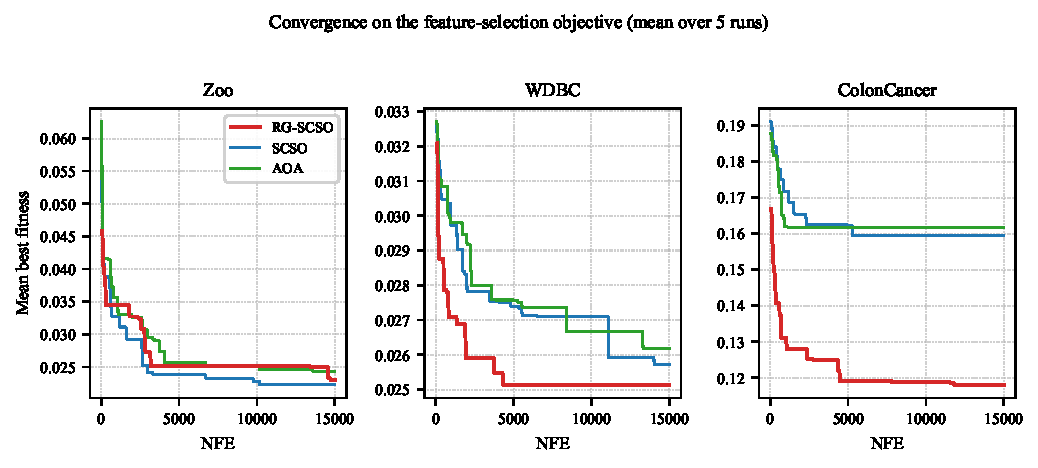
\includegraphics[width=0.92\textwidth]{convergence_fs.pdf}
\caption{Mean best fitness versus iteration, RG-SCSO vs.\ SCSO vs.\ AOA, on
Zoo (16 features), WDBC (30 features), and ColonCancer (2000 features), mean
over 5 runs, on the actual feature-selection objective (illustrative, not a
new statistical claim). On Zoo the three algorithms converge along
essentially the same trajectory. On WDBC and ColonCancer, RG-SCSO both
converges faster and plateaus at a lower (better) fitness than SCSO or AOA,
which themselves plateau early at a distinctly worse value rather than
continuing to close the gap with more iterations; the difference grows with
dimensionality.}
\label{fig:convfs}
\end{figure}

We also test whether relevance guidance makes RG-SCSO preferentially retain
high mutual-information features. Because a subset of size $|S|$ overlaps the
top-$|S|$ mutual-information features at a chance rate of $|S|/N$, we report a
size-fair enrichment (Fig.~\ref{fig:mech}), the fraction of selected
features in the top-$|S|$ set divided by this chance level. RG-SCSO's subset
is enriched above chance on both gene-expression sets, whereas the
relevance-agnostic SCSO sits at chance, evidence consistent with the
relevance field driving the smaller and more accurate subsets, though
enrichment alone is correlational. A direct causal test, detailed in
Supplementary Information, permutes the field's feature identities while
preserving its
value distribution: the permuted field yields no significant accuracy
difference from the real field on three of five datasets, a significant but
negligible-effect difference on Leukemia, and a clear difference only on
ColonCancer, while inverting the field's sign is significantly worse than
both on every dataset. The relevance field's direction and scale therefore
matter consistently; the exact per-feature ranking within it matters
demonstrably on only one of five datasets, a materially weaker causal claim
than the enrichment analysis alone would suggest.

\subsection{Threshold sensitivity}
The 0.5 preferred-bit threshold that separates preferred from disfavored
bits (Methods) is a convenience, not a theoretically grounded neutral point.
This sweep ($\tau\in\{0.4,0.5,0.6\}$, 30 independent runs per cell, same
protocol and datasets as the main ablation) tests whether that choice is at
least empirically reasonable. No single $\tau$ dominates uniformly:
$\tau=0.5$, the value deployed throughout this paper, attains the highest
accuracy on two of five datasets; mean selected-feature count falls
monotonically as $\tau$ increases on every dataset, at a modest,
dataset-dependent, non-uniform accuracy cost.

\begin{table}[t]
\centering
\caption{Threshold sensitivity ($\tau\in\{0.4,0.5,0.6\}$ replacing the fixed 0.5 preferred-bit threshold in Eq.~(2); 30 independent runs per cell, same protocol and datasets as the main ablation). Highest accuracy per dataset in bold. No single $\tau$ dominates uniformly: $\tau=0.5$, the value deployed throughout this paper, attains the highest accuracy on two of five datasets; mean selected-feature count falls monotonically as $\tau$ increases on every dataset, at a modest, dataset-dependent, non-uniform accuracy cost. $\Phi$ is the Nogueira stability index (Supplementary Information gives the full feature-selection stability comparison across algorithms).}
\label{tab:threshold}
\footnotesize
\begin{tabular}{lcccc}
\toprule
Dataset & $\tau$ & Mean Acc. & Mean \#Feat. & $\Phi$ \\
\midrule
\multirow{3}{*}{ColonCancer} & 0.4 & 0.8704 & 702.5 & 0.009 \\
 & 0.5 & \textbf{0.8809} & 563.1 & 0.014 \\
 & 0.6 & 0.8802 & 544.5 & 0.012 \\
\midrule
\multirow{3}{*}{Leukemia} & 0.4 & 0.9860 & 1205.4 & 0.011 \\
 & 0.5 & 0.9860 & 939.7 & 0.015 \\
 & 0.6 & \textbf{0.9864} & 927.6 & 0.012 \\
\midrule
\multirow{3}{*}{Sonar} & 0.4 & 0.8920 & 20.4 & 0.082 \\
 & 0.5 & \textbf{0.8940} & 19.1 & 0.088 \\
 & 0.6 & 0.8916 & 17.1 & 0.093 \\
\midrule
\multirow{3}{*}{WDBC} & 0.4 & \textbf{0.9795} & 13.2 & 0.193 \\
 & 0.5 & 0.9794 & 11.8 & 0.190 \\
 & 0.6 & 0.9791 & 11.1 & 0.163 \\
\midrule
\multirow{3}{*}{Zoo} & 0.4 & \textbf{0.9811} & 7.5 & 0.510 \\
 & 0.5 & 0.9808 & 7.3 & 0.541 \\
 & 0.6 & 0.9794 & 6.3 & 0.661 \\
\bottomrule
\end{tabular}
\end{table}


\begin{figure}[htbp]
\centering
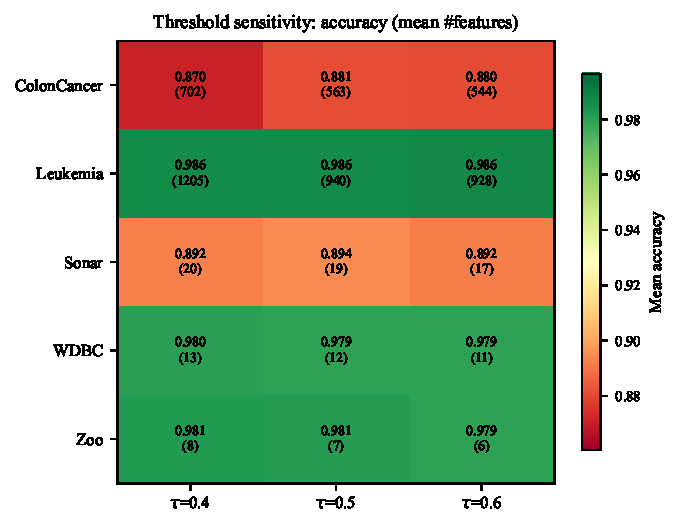
\includegraphics[width=0.55\textwidth]{threshold_heatmap.pdf}
\caption{Mean held-out accuracy (color) and mean number of selected features
(in parentheses) across the three preferred-bit thresholds tested
($\tau\in\{0.4,0.5,0.6\}$), one row per dataset. Accuracy is essentially
flat across thresholds on every dataset (largest swing 0.011, ColonCancer
$\tau{=}0.4$ vs.\ $\tau{=}0.5$), while the selected-feature count falls
monotonically as $\tau$ increases on all five datasets, confirming
$\tau=0.5$ is not a fragile choice.}
\label{fig:threshheat}
\end{figure}

\subsection{Comparison with classical selectors}
\label{sec:classical}
RQ4 asks how robust the mechanism is across classifiers, relevance priors, and dataset dimensionalities; this subsection and Table~\ref{tab:classifierrobust} answer it directly. Table~\ref{tab:classic} compares RG-SCSO across the full 18-dataset benchmark against five classical filter, embedded, and wrapper selectors -- mutual-information thresholding, mRMR, ReliefF, LASSO, and sequential forward selection -- and a Concrete-Autoencoder deep feature selector~\cite{{concreteae}}, under the identical stratified 5-fold KNN evaluator. RG-SCSO attains the best accuracy of all methods on 12 of 18 datasets. Across the benchmark it is significantly more accurate (Holm-corrected Wilcoxon signed-rank over the 18 datasets) than mutual-information thresholding, sequential forward selection, mRMR, and LASSO (all Holm $p<0.05$); the one classical selector it does not significantly beat is ReliefF, which it still leads on 13 of 18 datasets ($p=0.2$). The Concrete-Autoencoder baseline, matched to RG-SCSO's per-dataset subset size, is the weakest selector on the small-sample datasets tested, consistent with deep reconstruction objectives needing far more than the 50--455 training instances these benchmarks provide. The exceptions to RG-SCSO's lead are informative and concentrated: on the two gene-expression ($p\gg n$) datasets a classical LASSO baseline attains higher accuracy with far fewer features on both Leukemia (99.8\% at 23 features vs.\ RG-SCSO's 98.6\% at 940) and ColonCancer (95.7\% at 64 vs.\ 88.1\% at 563), with mRMR competitive on both; and on four combinatorial or categorical datasets (TicTacToe, M-of-n, KrVsKpEW, WaveformEW) a classical method edges it by at most 1.7 accuracy points. RG-SCSO's advantage is thus broad but not universal: clearest on datasets without extreme $p\gg n$ structure, where on ultra-high-dimensional gene-expression data a computationally far cheaper embedded method such as LASSO is a strong, arguably preferable, alternative. A remaining question is whether this parsimony mechanism is an artifact of the KNN wrapper used throughout; Table~\ref{tab:classifierrobust} answers it directly, extending the same relevance-guided search to SVM and Random Forest wrappers. The advantage over a no-prior baseline is not a KNN artifact, though it is a more consistent parsimony gain than an accuracy one under Random Forest specifically, and the ReliefF-prior degradation already established above reproduces under every wrapper tested.

\begin{sidewaystable}[t]
\centering
\caption{Full 18-dataset comparison of RG-SCSO against five classical filter/embedded/wrapper selectors and a Concrete-Autoencoder deep feature selector (CAE), replacing the earlier five-dataset pilot; accuracy with mean selected-feature count in parentheses, 30 runs each, identical evaluator (stratified 5-fold KNN) throughout, \textbf{bold} = best accuracy per dataset. RG-SCSO attains the best accuracy of all methods on 12 of 18 datasets. Across the benchmark it is significantly more accurate (Holm-corrected Wilcoxon signed-rank over the 18 datasets) than MI-thr ($p<0.001$), SFS ($p=0.002$), mRMR ($p=0.017$), LASSO ($p=0.047$); the one classical method it does not significantly beat is ReliefF (better on 13/18, $p=0.20$). The CAE baseline, matched to RG-SCSO's per-dataset subset size, is the weakest selector on the small-sample datasets tested, consistent with deep reconstruction objectives needing more data than these 50--455-instance benchmarks provide. LASSO and mRMR remain the strongest competitors on the two gene-expression ($p\gg n$) sets.}
\label{tab:classic}
\scriptsize
\setlength{\tabcolsep}{3.5pt}
\begin{tabular}{lccccccc}
\toprule
Dataset & RG-SCSO & LASSO & mRMR & ReliefF & SFS & MI-thr & CAE \\
\midrule
Diabetes & \textbf{0.760 (5)} & 0.735 (8) & 0.739 (7) & 0.745 (5) & 0.741 (7) & 0.695 (1) & 0.697 (5) \\
BreastEW & \textbf{0.974 (4)} & 0.968 (9) & 0.971 (7) & 0.972 (6) & 0.970 (8) & 0.965 (6) & 0.946 (4) \\
TicTacToe & 0.820 (7) & \textbf{0.847 (9)} & \textbf{0.847 (9)} & \textbf{0.847 (9)} & 0.788 (8) & 0.653 (1) & 0.738 (6) \\
HeartDisease & \textbf{0.849 (5)} & 0.821 (12) & 0.825 (11) & 0.829 (10) & 0.808 (12) & 0.740 (1) & 0.753 (5) \\
M-of-n & 0.994 (6) & \textbf{1.000 (6)} & 0.965 (8) & \textbf{1.000 (6)} & 0.868 (12) & 0.664 (1) & 0.712 (6) \\
Vote & \textbf{0.974 (3)} & 0.970 (1) & 0.970 (1) & 0.970 (1) & 0.924 (15) & 0.968 (1) & 0.841 (3) \\
Zoo & \textbf{0.981 (7)} & 0.888 (11) & 0.961 (11) & 0.965 (11) & 0.941 (15) & 0.753 (2) & 0.871 (6) \\
Lymphography & \textbf{0.865 (8)} & 0.823 (17) & 0.836 (13) & 0.862 (12) & 0.815 (17) & 0.695 (1) & 0.769 (7) \\
GermanCredit & \textbf{0.761 (8)} & 0.741 (20) & 0.744 (15) & 0.747 (13) & 0.744 (19) & 0.673 (1) & 0.691 (7) \\
Parkinsons & \textbf{0.962 (8)} & 0.912 (12) & 0.924 (9) & 0.940 (13) & 0.904 (21) & 0.867 (1) & 0.884 (7) \\
SpectEW & \textbf{0.859 (9)} & 0.810 (14) & 0.819 (10) & 0.836 (9) & 0.800 (21) & 0.699 (1) & 0.780 (8) \\
WDBC & \textbf{0.979 (12)} & 0.962 (20) & 0.972 (17) & 0.968 (13) & 0.967 (25) & 0.943 (10) & 0.952 (10) \\
IonosphereEW & \textbf{0.914 (8)} & 0.844 (31) & 0.905 (3) & 0.899 (4) & 0.860 (25) & 0.822 (1) & 0.862 (7) \\
KrVsKpEW & 0.943 (15) & 0.936 (32) & 0.923 (26) & \textbf{0.954 (15)} & 0.949 (25) & 0.522 (1) & 0.614 (12) \\
WaveformEW & 0.820 (16) & 0.812 (26) & 0.786 (23) & \textbf{0.837 (15)} & 0.812 (25) & 0.503 (1) & 0.786 (11) \\
Sonar & \textbf{0.894 (19)} & 0.808 (59) & 0.852 (18) & 0.820 (8) & 0.822 (25) & 0.686 (1) & 0.787 (16) \\
ColonCancer & 0.881 (563) & \textbf{0.957 (64)} & 0.907 (6) & 0.907 (11) & 0.902 (25) & 0.836 (3) & 0.794 (324) \\
Leukemia & 0.986 (940) & \textbf{0.998 (23)} & 0.989 (6) & 0.978 (10) & 0.981 (25) & 0.963 (30) & 0.892 (419) \\
\bottomrule
\end{tabular}
\end{sidewaystable}


\begin{table}[tb]
\centering
\caption{Robustness across classifier wrappers and relevance priors, averaged over five representative datasets (Zoo, Sonar, WDBC, ColonCancer, Leukemia; KNN/SVM use the main study's 30 independent runs per cell; Random Forest uses a reduced 10, given its far higher per-evaluation cost, disclosed rather than matched artificially). Per-dataset detail for all three wrappers is given in Supplementary Information. Fewest features per wrapper in bold.}
\label{tab:classifierrobust}
\footnotesize
\begin{tabular}{llcc}
\toprule
Wrapper & Method & Mean Acc. & Mean \#Feat. \\
\midrule
\multirow{3}{*}{KNN (30 runs)} & \textbf{RG-SCSO (MI)} & 0.9442 & \textbf{308.2} \\
 & RG-SCSO (ReliefF) & 0.9380 & 565.8 \\
 & bSCSO (no prior) & 0.9350 & 545.1 \\
\midrule
\multirow{3}{*}{SVM (30 runs)} & \textbf{RG-SCSO (MI)} & 0.9489 & \textbf{299.1} \\
 & RG-SCSO (ReliefF) & 0.9476 & 555.2 \\
 & bSCSO (no prior) & 0.9468 & 537.5 \\
\midrule
\multirow{3}{*}{RF (10 runs)} & \textbf{RG-SCSO (MI)} & 0.9521 & \textbf{313.1} \\
 & RG-SCSO (ReliefF) & 0.9514 & 571.6 \\
 & bSCSO (no prior) & 0.9505 & 546.2 \\
\bottomrule
\end{tabular}
\end{table}


\begin{figure}[htbp]
\centering
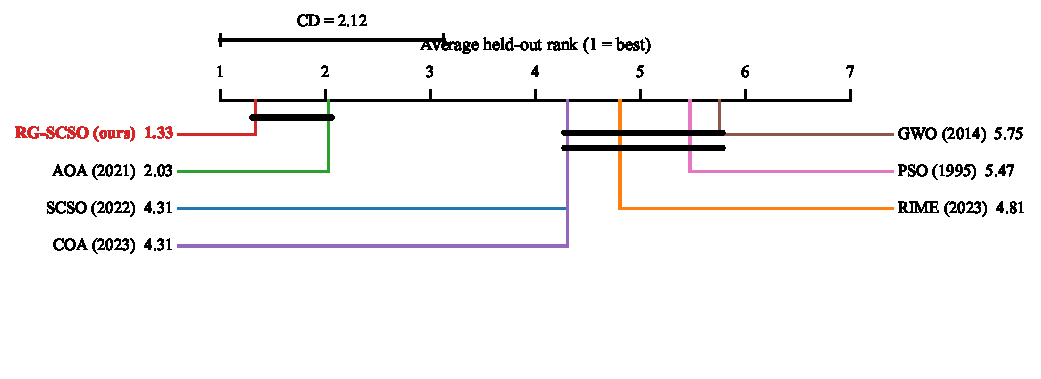
\includegraphics[width=0.92\textwidth]{cd_diagram_heldout.pdf}
\caption{Critical-difference (Nemenyi) diagram at $\alpha=0.05$ over the
held-out ranking (Table~\ref{tab:heldout}); algorithms not joined by a bar
differ significantly in mean held-out rank. RG-SCSO attains the best mean rank
(1.33) and AOA the second (2.03); the remaining five algorithms cluster
between 4.31 and 5.75. The critical difference is $\mathrm{CD}=2.12$ (7
algorithms, 18 datasets), so RG-SCSO and AOA are statistically
indistinguishable from each other yet both separate from the rest. The
corresponding in-sample diagram appears in Supplementary Fig.~S6.}
\label{fig:cd}
\end{figure}

\begin{figure}[htbp]
\centering
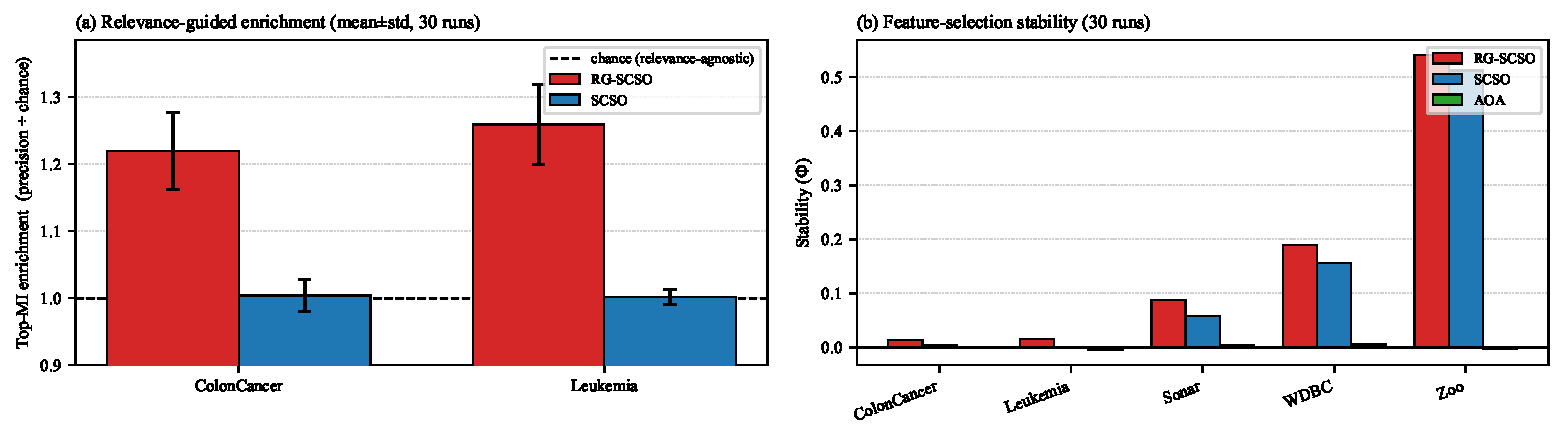
\includegraphics[width=0.95\textwidth]{mechanism.pdf}
\caption{Mechanism evidence. (a) Size-fair top-MI enrichment on the two
gene-expression sets (selection precision divided by the chance level
$|S|/N$; mean over 30 runs, error bars = std): RG-SCSO enriches its subset
1.22--1.26$\times$ above chance (ColonCancer, Leukemia respectively),
whereas the relevance-agnostic SCSO sits at essentially chance (lift 1.00
on both). (b) Feature-selection stability (Nogueira $\Phi$, 30 runs) across
all five representative datasets: RG-SCSO attains a higher $\Phi$ than
same-family SCSO on every dataset (e.g., 0.541 vs. 0.512 on Zoo, 0.19 vs.
0.157 on WDBC), clearest on the three lower-dimensional sets, but
both are close to the near-zero level expected by chance on the two
gene-expression sets (RG-SCSO $\Phi\approx$0.014--0.015), where AOA's
near-zero $\Phi$ reflects that it selects nearly every
available feature rather than genuine instability.}
\label{fig:mech}
\end{figure}

\FloatBarrier
\section{Discussion}
These results trace washout, a concrete failure mode of
transfer-function-based binary feature selection, to its source, and cure it
by moving the relevance signal directly inside the binarization operator
rather than upstream of it in the objective or the initialization. The formal
result motivating this design (Methods) is a diagnostic bound: it explains why
continuous-space enhancements fail at the binarization boundary, but it is not
a convergence guarantee for RG-SCSO itself. The underlying recipe, a filter
prior coupled to a wrapper search with memetic refinement, is a known
combination in the feature-selection literature. What is new is the injection
point, together with a stringent evaluation protocol: budget-matching, a
leak-free hold-out, cross-classifier and cross-prior robustness, and an
explicit exploration-safety diagnostic. We report parsimony, not raw accuracy,
as the transferable outcome of this choice.

Several boundaries delimit what these results establish. RG-SCSO inherits
SCSO's continuous search dynamics unchanged, and the RMS rule carries a risk
of its own: bias the flip probability too strongly and confidently classified
bits can freeze in place, draining population diversity. We measured this
directly rather than assuming it away: at an aggressive stress-test bias the
risk is real and grows with dimensionality, but the conservative $\gamma=0.5$
this paper deploys keeps the frozen-bit fraction below
1.1\% throughout
the run on every dataset tested. We also tested whether UMR's benefit
specifically requires targeting relevance-uncertain features, or only the
extra evaluation budget it spends, by replacing its targeted $K$-feature
selection with $K$ uniformly random features at matched NFE (Supplementary
Information). This untargeted control significantly outperforms targeted
UMR on both accuracy and feature count on the two gene-expression datasets,
where UMR's contribution is largest (ColonCancer: 90.6\% vs.\ 88.1\%
accuracy, 214 vs.\ 563 features; Leukemia: 423 vs.\ 940 features at
statistically indistinguishable accuracy), and ties it on the other three.
UMR's value over no memetic step at all remains real (Table~3); on the
datasets where that value is largest, however, it does not depend on
targeting relevance-uncertain features specifically, a more modest claim
than ``uncertainty-targeted'' on its own implies. The relevance field is
built from a single filter statistic. Swapping in a ReliefF prior exposes a
genuine limitation rather than confirming the mechanism: the parsimony
advantage disappears entirely (Supplementary Information). RG-SCSO's
compactness therefore depends on a prior that drives uninformative features
below the neutral point, not on the mere presence of a relevance signal. This dependence, together with the
$O(dn\log n)$ one-time cost of the mutual-information prior amortized
against the wrapper's $N+K$ per-iteration evaluations, is why we scope the
scalability claim to the wrapper cost dominating overall runtime as feature
dimensionality grows (full per-dataset wall-clock cost is in Supplementary
Information) rather than to any runtime advantage over same-budget
baselines, which we do not claim.

The main
objective is also a KNN wrapper. Under SVM, tested directly on
16 of the 18 datasets, and under Random Forest on
the same five-dataset subset as Table~\ref{tab:classifierrobust}, the
parsimony advantage is not a KNN artifact. Under Random Forest specifically it
is a more consistent gain in subset size than in accuracy, and the
ReliefF-prior degradation established above reproduces under every wrapper
tested. The selected subset is smaller and
more consistent in size than competing algorithms', but not necessarily
more consistent in identity: a feature-selection stability index shows
RG-SCSO more stable run to run than same-family SCSO on every dataset,
clearest on the three lower-dimensional sets, yet on both gene-expression
datasets RG-SCSO's own stability is itself close to the level expected by
chance, so a much smaller subset there is not a materially more repeatable
one (Fig.~\ref{fig:mech}b; Supplementary Information gives the full
per-dataset breakdown for both checks).

This wrapper search is itself compute-intensive; absolute wall-clock cost
per run, for every algorithm tested, is reported in full in Supplementary
Information rather than only argued qualitatively. A genuine outer-fold
nested cross-validation pilot on three datasets, also in Supplementary
Information, is directionally consistent with the single-split held-out
estimate above, though underpowered at five runs per cell to confirm
significance independently.

External validity has its own limits: the benchmark spans
8 to 3571 features across biomedical, gene-expression, and
categorical domains drawn from a single curated family of UCI and standard
microarray sets. Its top end (3571 features, Leukemia) is still an order
of magnitude below the $10^4$--$10^5$-feature omics and high-dimensional text
regimes where a binary-native, relevance-guided operator should matter most,
so behaviour at that scale is extrapolated, not measured; a genuine
$>$$10^4$-feature evaluation is deferred to future work because a full
seven-optimizer, 30-run wrapper study at that dimensionality is compute-bound
by the $O(N\,\mathrm{max\_nfe})$ KNN fitness evaluations rather than by the
relevance mechanism itself, and lies outside this study's fixed budget. The
relevance field
itself is not perfectly stable on the smallest, highest-dimensional
datasets: a bootstrap resampling analysis, reported in Supplementary
Information, shows markedly lower rank stability of the mutual-information
field on the two gene-expression sets than on the three lower-dimensional
benchmarks, a risk the classical-baseline comparison above makes concrete
rather than theoretical.

Finally, the accuracy claim is scoped, not universal: against
binary particle-swarm and grey-wolf optimizers carrying published adaptive
transfers, and against same-family binary SCSO selectors, RG-SCSO does not
lead on accuracy, and on the two gene-expression datasets specifically a
classical LASSO baseline outperforms RG-SCSO outright, so we do
not claim a practical advantage for RG-SCSO on ultra-high-dimensional,
small-sample data; we scope its transferable benefit to parsimony on
datasets without that extreme structure. These boundaries are gathered
together, with the future work they motivate, in Conclusion below.

\FloatBarrier
\section{Conclusion}
The results support RG-SCSO as a relevance-guided binary
feature-selection method whose primary advantage is improved subset
parsimony with competitive predictive performance under the tested
conditions: across 18 benchmark datasets it selects the
second-smallest feature subsets of any method evaluated, trailing only COA,
while attaining the best mean held-out accuracy among all seven algorithms
compared, under a fixed, budget-matched, leak-free evaluation protocol
(RQ1, RQ2).

This advantage is not universal, and the boundaries established in
Discussion above are real constraints on the claim, not caveats to be
read past. Against optimizers carrying published adaptive continuous-space
transfers, and against same-family binary SCSO selectors, RG-SCSO does not
lead on accuracy. On the two extreme $p\gg n$ gene-expression datasets tested,
a classical LASSO baseline outperforms it outright on both accuracy and
feature count. Its dependence on the underlying relevance prior is genuine:
replacing mutual information with a ReliefF prior removes the parsimony
advantage entirely. The 0.5 preferred-bit threshold, while empirically
reasonable across the range tested, is not a uniformly optimal choice. And the
benchmark itself, though spanning 8--3571 features across
biomedical, gene-expression, and categorical domains, is drawn from a single
curated family of datasets, so behavior on ultra-high-dimensional omics data
of $10^4$--$10^5$ features is extrapolated rather than measured.

In practical terms, RG-SCSO is a drop-in replacement for the binarization
step of any SCSO-based wrapper, adding only a small, fixed set of
hyperparameters (the modulation strength $\gamma$, the preferred-bit
threshold $\tau$, and the memetic budget $K$) that this paper shows are
not fragile choices; its main practical payoff is a smaller,
cheaper-to-store and cheaper-to-deploy feature subset at accuracy that
matches or exceeds the swarm-based selectors it was compared against.

\textbf{Future work} includes: (i) adaptive, data-driven selection of the
preferred-bit threshold, for example via cross-validation or an
entropy-based criterion, rather than a fixed value; (ii) an explicit
multi-objective formulation that traces an accuracy-parsimony Pareto front
rather than a single weighted objective; (iii) extending the
relevance-modulated binarization mechanism to other swarm optimizers, such
as WOA, HHO, or SMA, to test whether the injection-point argument
generalizes beyond SCSO; (iv) evaluation at larger scale, on datasets
exceeding $10^4$ features, where a relevance-guided, binary-native operator
should be especially valuable; and (v) alternative relevance priors beyond
mutual information and ReliefF, such as SHAP-based, mRMR, or learned
priors, to test whether the mechanism's benefit is specific to the prior
used here or transfers to others.

\FloatBarrier
\section{Methods}
\label{sec:method}

\begin{algorithm}[!t]
\caption{RG-SCSO for binary feature selection}
\label{alg:main}
\begin{algorithmic}[1]
  \REQUIRE training partition $(X,y)$ (never the held-out fold; see Methods
    below for the fold-honest protocol); population size $N$; iterations
    $T_{\max}$; budget $\mathrm{max\_nfe}$; memetic size $K$; bias
    strength $\gamma$
  \ENSURE best feature mask $b^\ast$
  \STATE $\rho_j \leftarrow$ normalized mutual information $I(X_j;y)$,
    computed on $(X,y)$ only, $\forall j$ \hfill$\triangleright$ static
    relevance field
  \STATE $\forall j$: preferred bit $\hat{b}_j \leftarrow \mathbf{1}[\rho_j>0.5]$;
    strength $s_j \leftarrow 2|\rho_j-0.5|$
  \STATE initialize positions $x_i \sim \mathcal{U}(-1,1)^d$, $i=1,\dots,N$;
    form the initial masks by sign only ($b_i=1$ if $x_i>0$, else $0$);
    evaluate; set $b^\ast$ \hfill$\triangleright$ the relevance-modulated flip
    rule (lines~8--11) is \emph{not} applied at initialization
  \WHILE{$\mathrm{nfe} < \mathrm{max\_nfe}$}
    \STATE $R \leftarrow S_M\,(1-t/T_{\max})$ \hfill$\triangleright$ sensitivity range contracts
    \FOR{each agent $i=1,\dots,N$}
      \STATE update $x_i$ by the SCSO position rule using range $R$
      \FOR{each feature $j$}
        \STATE $p_{\text{base}} \leftarrow |\tanh(x_{ij})|$ \hfill$\triangleright$ base transfer $T(x_{ij})$
        \STATE $p_j \leftarrow p_{\text{base}}\,(1+\gamma s_j)$ if the flip moves bit $j$ toward
          $\hat{b}_j$, else $p_{\text{base}}\,(1-\gamma s_j)$
        \STATE flip bit $j$ with probability $\mathrm{clip}(p_j,0,1)$
      \ENDFOR
      \STATE evaluate mask; update $b^\ast$ if improved
    \ENDFOR
    \STATE $U \leftarrow K$ features whose $\rho_j$ is closest to $0.5$
      \hfill$\triangleright$ UMR on uncertain bits
    \FOR{each $j \in U$}
      \STATE flip bit $j$ of $b^\ast$; keep the flip only if fitness improves
    \ENDFOR
  \ENDWHILE
  \RETURN $b^\ast$
\end{algorithmic}
\end{algorithm}

\subsection{Problem formulation}
Let a candidate subset be a binary mask $b\in\{0,1\}^d$. The objective is
\begin{equation}
  f(b) = 0.99\,(1-\mathrm{Acc}(b)) + 0.01\,\frac{|b|}{d},
  \label{eq:fitness}
\end{equation}
where $\mathrm{Acc}(b)$ is the stratified 5-fold KNN accuracy ($k=5$) using only
the selected features. Every baseline in this study optimizes this same
objective with the same 0.01 cardinality weight. RG-SCSO is granted no
structural advantage on subset size from the fitness function itself, so any
parsimony gap reported below reflects the search mechanism, not a differently
weighted objective. SCSO governs its search with the sensitivity range
$R(t)=S_M - S_M\,t/T$ ($S_M=2$), which RG-SCSO retains while replacing the
binarization and adding a relevance field.

\subsection{Theoretical motivation: transfer-function washout}
\label{sec:washout}
Consider any binary-native optimizer that keeps a real-valued position and
binarizes coordinate $j$ through a transfer $T:\mathbb{R}\to[0,1]$. A
continuous-space enhancement can influence the retained subset only by
perturbing a coordinate, $x_j\mapsto x_j+\delta_j$; its entire effect on the
discrete decision is the induced change in probability
$\Delta_j=T(x_j+\delta_j)-T(x_j)$.

\begin{lemma}[Leverage bound]
Let $T:\mathbb{R}\to[0,1]$ be Lipschitz and piecewise continuously
differentiable. If a coordinate-space enhancement perturbs $x_j$ by $\delta_j$,
$|\Delta_j|\le\|T'\|_\infty\,|\delta_j|$, where $\|T'\|_\infty$ is the largest
slope $T$ attains between $x_j$ and $x_j+\delta_j$. For the two standard
transfers $\|\sigma'\|_\infty=\tfrac14$ and $\||\tanh|'\|_\infty=1$, and each
slope decays away from the origin; in a flat region, where
$\|T'\|_\infty\le\varepsilon$, the leverage collapses to
$|\Delta_j|\le\varepsilon\,|\delta_j|$ (proof in Supplementary Information).
\end{lemma}
\noindent\textbf{Remark (why RG-SCSO is exempt).} RG-SCSO breaks the premise
of the lemma: instead of routing information through the coordinate, it
modulates the flip probability directly at the transfer output,
$\Delta_j=\pm\,\gamma\,s_j\,V(x_j)$, independent of $T'$. The base transfer
$T$ still appears inside RG-SCSO's own rule as one multiplicative factor
(Eq.~\ref{eq:rms} below), but Proposition~2, which follows next,
characterizes only the base operator's transition probability
$T(x_j^{(t)})$ itself, not RG-SCSO's realized flip probability $p_j$, which
this Remark has just shown is exempt from Lemma~1's bound by construction.

\begin{proposition}[Transition probability under the base V-shaped transfer]
This proposition characterizes only the base, unmodulated V-shaped transfer
introduced above (the NoRMS reference operator used in the ablation);
RG-SCSO's own operator is exempt from it by construction, per the Remark
above. Under this unmodulated V-shaped binarization rule, bit $j$
flips at iteration $t$ with probability $T(x_j^{(t)})$, so the base
operator's one-step bit-transition probability coincides with $T$,
$P_{\text{base}}\big(b_j^{(t+1)}\ne b_j^{(t)}\mid x_j^{(t)}\big)=T(x_j^{(t)})$.
Lemma~1's
bound on $\Delta_j$ is therefore, without further assumption, already a
bound on the one-step change in the base operator's transition probability,
and this bound
composes linearly over $N$ repeated samples of the same bit in the flat,
saturated regime (proof in Supplementary Information). For RG-SCSO itself,
this base probability $T(x_j^{(t)})$ is subsequently modulated by the
relevance-modulated rule $p_j$ of Eq.~\ref{eq:rms} below, so RG-SCSO's
actual one-step transition probability is $p_j$, not $T(x_j^{(t)})$ alone.
This is a local,
one-step-composable sensitivity bound, not a convergence guarantee or a
proof that continuous-space enhancements are ineffective; the full scope
discussion is in Supplementary Information.
\end{proposition}

\subsection{The RG-SCSO mechanism}
Given the updated position $x_j$, the base flip probability uses a V-shaped
transfer $V(x_j)=|\tanh(x_j)|$. With relevance $\rho_j\in[0,1]$, preferred bit
$b^\ast_j=\mathbf{1}[\rho_j>0.5]$ and strength $s_j=2|\rho_j-0.5|\in[0,1]$,
the flip probability is biased toward $b^\ast_j$,
\begin{equation}
  p_j = \mathrm{clip}\!\Big(|\tanh(x_j)|\,\big(1+\gamma\,\sigma_j\,s_j\big),\,0,\,1\Big),
  \label{eq:rms}
\end{equation}
where $\sigma_j=+1$ if the flip moves bit $j$ toward $b^\ast_j$ and $\sigma_j=-1$
otherwise. Setting $\gamma=0$ recovers a plain V-shaped operator (the NoRMS
ablation). The 0.5 threshold that separates preferred from disfavored bits is
a convenience, not a theoretically grounded neutral point: with
$\rho_j=I(X_j;y)/H(y)$, the value at which a feature stops being informative
depends on the number of classes, the label entropy, the sample size, and
the specific MI estimator used, none of which are normalized away by the
$H(y)$ division alone. The Discussion shows this dependence is not merely
theoretical: the method's compactness is tied to how the chosen relevance
statistic happens to place features around 0.5, not to the threshold
itself. A threshold sweep ($\tau\in\{0.4,0.5,0.6\}$, Results
Section~\ref{sec:ablation}) supports this choice as reasonable rather than
arbitrary: $\tau=0.5$ attains the highest accuracy on two of five datasets
tested, and every value trades a modest, dataset-dependent accuracy shift
for a monotonic reduction in feature count as $\tau$ increases, with no
single value dominating uniformly.

The field $\rho$ that drives this mechanism is, in the final method, the
static prior $\rho_{\mathrm{static}}=\mathrm{clip}(\mathrm{MI}(f_j;y)/H(y),0,1)$,
a normalized mutual-information filter score~\cite{mrmr,kraskov} computed once
from the data; an online extension adding an EMA credit-assignment term from
accepted fitness improvements was examined and dropped, as the ablation
shows no accuracy gain on any dataset. A second, smaller component,
uncertainty-targeted memetic refinement (UMR), spends a fixed local-search
budget where this prior is least decisive: each iteration, the $K$ features
whose relevance is closest to $0.5$ are greedily flipped on the incumbent
best mask~\cite{neri} and the flip is kept only if fitness improves.

\subsection{Algorithm and computational cost}
Every fitness evaluation, whether from population moves, memetic probes, or
initialization, is counted against a single budget $\mathrm{max\_nfe}=\mathrm{pop\_size}\times
\mathrm{max\_iter}=15000$, identical to the baselines, so UMR grants no extra
evaluations (Algorithm~\ref{alg:main}).

The per-iteration cost is dominated by the $N+K$ wrapper evaluations, each a
KNN fit under fixed folds; the mutual-information prior adds a one-time
$O(dn\log n)$ preprocessing cost (the nearest-neighbor MI
estimator~\cite{kraskov}), amortized against the wrapper evaluations. RG-SCSO
is thus asymptotically no more expensive than base SCSO apart from the $K$
extra probes. In wrapper feature selection generally, classifier-based
fitness evaluation, not the search mechanism itself, dominates overall
computational cost as feature dimensionality grows; per-dataset wall-clock
measurements across the full 8--3571-feature range tested
(Supplementary Information) are consistent with this expectation, and we
make no runtime-speedup claim for RG-SCSO over same-budget baselines.

\subsection{Datasets, baselines, and protocol}
The benchmark spans 18 preprocessed datasets of 8 to
3571 features across biomedical, gene-expression, and categorical
domains, full characteristics in Supplementary Table~S1.

We benchmark against six baselines: SCSO (base)~\cite{scso},
AOA~\cite{aoa}, CoatiOA~\cite{coa}, GWO~\cite{gwo}, PSO~\cite{pso}, and
RIME~\cite{rime}. The protocol is preregistered and locked prior to the full
run. All algorithms share: population 30, 500 iterations, 30 independent
runs, seed $=42+\mathrm{run\_id}$ (paired across algorithms), KNN ($k=5$)
with stratified 5-fold cross-validation, search space $[-1,1]^d$, and the
fitness of~\eqref{eq:fitness}. Every baseline runs with its library-default
published hyperparameters, with only population size and evaluation budget
matched across methods; RG-SCSO's $\gamma$ and $K$ are likewise fixed before
the full run.

\subsection{Statistics and reproducibility}
Significance uses the paired Wilcoxon signed-rank test with Holm
correction~\cite{holm}, the Holm family formed \emph{per dataset}, at
$\alpha=0.05$. A tie denotes failure to reject $H_0$ (no significant
accuracy difference) at this threshold; it is not evidence of equivalence.
Effect sizes use Cohen's $d$ and rank-biserial $r$; overall comparison uses the
Friedman test with a critical-difference diagram~\cite{demsar}. The
experimental design was preregistered and version-controlled before the full
run and left unmodified after results were observed; all randomness is
seeded deterministically and shared across algorithms.

\section*{Author Contributions}
\textbf{Bui Quang Huy:} Conceptualization, Methodology, Software,
Validation, Formal analysis, Investigation, Data curation, Writing --
original draft, Writing -- review \& editing, Visualization, Supervision.
\textbf{Duong Minh Son:} Formal analysis, Writing -- review \& editing.

\section*{Statements and Declarations}

\subsection*{Funding}
No funding was received for this work.

\subsection*{Conflict of interest}
The authors declare no competing interests.

\subsection*{Ethical approval}
Not applicable. This study uses only publicly available benchmark datasets
(UCI and standard microarray sets) and involves no human participants,
human data, or animals.

\subsection*{Data Availability Statement}
The datasets analysed in this study are publicly available benchmarks (UCI
and standard microarray sets); Supplementary Table~S1 lists each source. The
source code, the locked preregistration, the per-run seeds, a complete
hyperparameter table, a pinned dependency list, and the raw per-run results
are available for review in an anonymized repository
(\url{https://anonymous.4open.science/r/RG-SCSO}) and will be deposited in a
public, citable repository with a permanent Zenodo DOI upon acceptance,
permitting bit-for-bit reproduction of every number reported in this paper.

% Note: sn-jnl.cls already sets \bibliographystyle{sn-basic} internally, so
% an explicit \bibliographystyle here would trigger BibTeX's "Illegal, another
% \bibstyle command" error; we deliberately omit it and only invoke
% \bibliography.
\bibliography{references}

\end{document}
